% ============================================================
% Partitions satisfaisantes dans les graphes
% Beamer presentation — Master 1 Algorithmique
% Auteur : Ivan LEJEUNE   |   Encadrant : Stéphane BESSY
% ============================================================



% ---------- Thème ----------
\usetheme{Madrid}
\usecolortheme{default}

% Palette principale (bleu UM + orange accent)
\definecolor{umblue}{RGB}{0,62,126}
\definecolor{umorange}{RGB}{220,100,30}
\definecolor{lightblue}{RGB}{200,220,245}
\definecolor{lightgray}{RGB}{245,245,245}

\setbeamercolor{palette primary}{bg=umblue, fg=white}
\setbeamercolor{palette secondary}{bg=umblue!80, fg=white}
\setbeamercolor{palette tertiary}{bg=umblue!60, fg=white}
\setbeamercolor{palette quaternary}{bg=umblue, fg=white}
\setbeamercolor{structure}{fg=umblue}
\setbeamercolor{frametitle}{bg=umblue, fg=white}
\setbeamercolor{title}{fg=white}
\setbeamercolor{section in toc}{fg=umblue}
\setbeamercolor{block title}{bg=umblue!90, fg=white}
\setbeamercolor{block body}{bg=lightblue!40}
\setbeamercolor{block title alerted}{bg=umorange, fg=white}
\setbeamercolor{block body alerted}{bg=umorange!15}
\setbeamercolor{block title example}{bg=umblue!60, fg=white}
\setbeamercolor{block body example}{bg=lightblue!25}

% ---------- Polices & encodage ----------
\usepackage[T1]{fontenc}
\usepackage[utf8]{inputenc}
% French accents handled via explicit commands

% ---------- Maths ----------
\usepackage{amsmath, amssymb, amsthm}
\usepackage{mathtools}

% ---------- TikZ (sans graphdrawing, qui necessite LuaTeX) ----------
\usepackage{tikz}
\usetikzlibrary{arrows.meta, positioning, calc}

% ---------- Divers ----------
\usepackage{xcolor}
\usepackage{listings}
\usepackage{hyperref}
\usepackage{booktabs}

% ---------- Macros ----------
\newcommand{\dint}{d_{\mathrm{int}}}
\newcommand{\dext}{d_{\mathrm{ext}}}

% ---------- Listings Python ----------
\lstset{
  language=Python,
  basicstyle=\ttfamily\tiny,
  keywordstyle=\color{umblue}\bfseries,
  commentstyle=\color{gray},
  stringstyle=\color{umorange},
  numbers=left,
  numberstyle=\tiny\color{gray},
  frame=single,
  backgroundcolor=\color{lightgray},
  breaklines=true,
  showstringspaces=false,
  tabsize=4
}

% ---------- Footline personnalisee ----------
\setbeamertemplate{footline}{%
  \leavevmode%
  \hbox{%
    \begin{beamercolorbox}[wd=.33\paperwidth,ht=2.25ex,dp=1ex,center]{palette primary}%
      \usebeamerfont{author in head/foot}Ivan LEJEUNE
    \end{beamercolorbox}%
    \begin{beamercolorbox}[wd=.34\paperwidth,ht=2.25ex,dp=1ex,center]{palette secondary}%
      \usebeamerfont{title in head/foot}Partitions satisfaisantes dans les graphes
    \end{beamercolorbox}%
    \begin{beamercolorbox}[wd=.33\paperwidth,ht=2.25ex,dp=1ex,right]{palette tertiary}%
      \usebeamerfont{date in head/foot}\insertshortdate{}\hspace*{1em}
      \insertframenumber{} / \inserttotalframenumber\hspace*{1ex}
    \end{beamercolorbox}%
  }%
  \vskip0pt%
}

% ---------- Navigation symbols ----------
\setbeamertemplate{navigation symbols}{}

% ============================================================
\title[Partitions satisfaisantes]{Partitions satisfaisantes dans les graphes}
\subtitle{Travail d'\'Etude et de Recherche --- Master 1 Algorithmique}
\author[I.\ Lejeune]{\textbf{Ivan LEJEUNE} \\ {\small Encadrant : St\'ephane BESSY}}
\institute[Universit\'e de Montpellier]{Universit\'e de Montpellier \\ Facult\'e des Sciences de Montpellier}
\date{25 mai 2026}
% ============================================================

\begin{document}

% ============================================================
%  TITRE
% ============================================================
\begin{frame}[plain]
  \titlepage
\end{frame}

% ============================================================
%  PLAN
% ============================================================
\begin{frame}{Plan}
  \tableofcontents
\end{frame}

% ============================================================
\section{Introduction et d\'efinitions}
% ============================================================

\begin{frame}{Contexte}
  \begin{block}{Cadre g\'en\'eral}
    Soit $G = (V, E)$ un graphe simple, non orient\'e, fini.
    \medskip

    On \'etudie l'existence d'une \alert{partition satisfaisante} de ses sommets : une notion qui formalise la coh\'esion interne au sein de sous-structures de graphes.
  \end{block}

  \bigskip

  \begin{definition}[Degr\'es interne et externe]
    Soit $(A,B)$ une partition de $V$ et $x \in V$.
    \begin{itemize}
      \item Si $x \in A$ : $\;\dint(x) = |N(x) \cap A|$, $\quad \dext(x) = |N(x) \cap B|$
      \item Si $x \in B$ : $\;\dint(x) = |N(x) \cap B|$, $\quad \dext(x) = |N(x) \cap A|$
    \end{itemize}
  \end{definition}
\end{frame}

\begin{frame}{Partition satisfaisante}
  \begin{definition}[Partition satisfaisante]
    Une partition $(A,B)$ de $V$ est \alert{satisfaisante} si pour tout $x \in V$ :
    \[
      \dint(x) \;\geq\; \dext(x)
    \]
    Un sommet v\'erifiant cette condition est dit \emph{satisfait}.

    \medskip
    Le probl\`eme de d\'ecision associ\'e est not\'e \textsc{Satisfactory Graph Partition}.
  \end{definition}

  \bigskip

  \begin{columns}[T]
    \column{0.52\textwidth}
    \begin{block}{Intuition}
      Chaque sommet doit avoir \emph{au moins autant} de voisins dans sa propre communaut\'e que dans l'autre.

      \medskip
      $\Rightarrow$ notion de \textbf{coh\'esion} ou \textbf{communaut\'e}.
    \end{block}

    \column{0.45\textwidth}
    \centering
    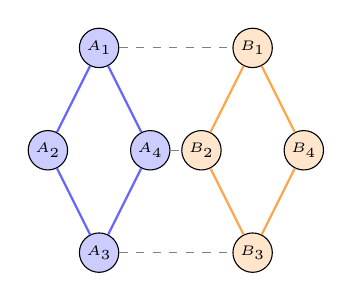
\begin{tikzpicture}[scale=0.65,
        every node/.style={circle, draw, minimum size=5mm, inner sep=1pt, font=\tiny}
      ]
      \node[fill=blue!20]   (A1) at (0,2)   {$A_1$};
      \node[fill=blue!20]   (A2) at (-1,0)  {$A_2$};
      \node[fill=blue!20]   (A3) at (0,-2)  {$A_3$};
      \node[fill=blue!20]   (A4) at (1,0)   {$A_4$};
      \node[fill=orange!20] (B1) at (3,2)   {$B_1$};
      \node[fill=orange!20] (B2) at (2,0)   {$B_2$};
      \node[fill=orange!20] (B3) at (3,-2)  {$B_3$};
      \node[fill=orange!20] (B4) at (4,0)   {$B_4$};
      \draw[blue!60, thick] (A1)--(A2)--(A3)--(A4)--(A1);
      \draw[orange!70, thick] (B1)--(B2)--(B3)--(B4)--(B1);
      \draw[gray, dashed] (A1)--(B1);
      \draw[gray, dashed] (A4)--(B2);
      \draw[gray, dashed] (A3)--(B3);
    \end{tikzpicture}
  \end{columns}
\end{frame}

% ============================================================
\section{Motivations et \'etat de l'art}
% ============================================================

\begin{frame}{Motivations}
  \begin{columns}[T]
    \column{0.32\textwidth}
    \begin{alertblock}{R\'eseaux sociaux \& biologiques}
      Sommets $=$ individus ou g\`enes ; ar\^etes $=$ interactions.

      \smallskip
      Une partition satisfaisante isole des \textbf{communaut\'es stables} o\`u l'activit\'e interne prime.
    \end{alertblock}

    \column{0.32\textwidth}
    \begin{alertblock}{Th\'eorie des jeux}
      Mod\'elise la \textbf{formation d'alliances d\'efensives} : un groupe $A$ est stable si chaque membre trouve plus de soutien en interne qu'il n'affronte de menaces externes.
    \end{alertblock}

    \column{0.32\textwidth}
    \begin{alertblock}{Intelligence artificielle}
      Pilier du \textit{clustering} non supervis\'e.

      \smallskip
      Densit\'e interne $>$ connectivit\'e externe $\Rightarrow$ meilleure \textbf{robustesse} pour la classification.
    \end{alertblock}
  \end{columns}
\end{frame}

\begin{frame}{\'Etat de l'art}
  \begin{block}{R\'ef\'erences principales}
    \begin{itemize}
      \item Bazgan, Tuza, Vanderpooten (2010) --- travaux fondateurs
      \item Yero \& Rodr\'{\i}guez-Vel\'azquez (2018) --- alliances d\'efensives
      \item Gaikwad, Maity, Tripathi (2020) --- algorithmes structurels
      \item B\"arnkopf, Nagy, Paulovics (2024) --- cas 5-r\'egulier et au-del\`a
    \end{itemize}
  \end{block}

  \medskip

  \begin{columns}[T]
    \column{0.48\textwidth}
    \begin{block}{R\'esultats de complexit\'e connus}
      \begin{itemize}
        \item \textbf{NP-complet} en g\'en\'eral
        \item \textbf{Polynomial} pour :
          \begin{itemize}
            \item graphes \`a clique-width born\'ee
            \item $\Delta(G) \leq 4$
          \end{itemize}
      \end{itemize}
    \end{block}

    \column{0.48\textwidth}
    \begin{exampleblock}{Notre approche}
      \begin{itemize}
        \item Construire des \textbf{contre-exemples} \`a la conjecture
        \item Identifier des \textbf{invariants structurels} minimaux bloquants
        \item Exp\'erimentation algorithmique sur les petits graphes
      \end{itemize}
    \end{exampleblock}
  \end{columns}
\end{frame}

% ============================================================
\section{R\'esultats pour les graphes $k$-r\'eguliers ($k \leq 4$)}
% ============================================================

\begin{frame}{La conjecture centrale}
  \begin{alertblock}{Conjecture (ouverte pour $k \geq 5$)}
    Pour tout entier $k$, tous les graphes $k$-r\'eguliers, \textbf{sauf un nombre fini d'exceptions}, admettent une partition satisfaisante.
  \end{alertblock}

  \bigskip

  \begin{block}{R\'eduction aux graphes connexes}
    \textbf{Proposition.} Tout graphe \emph{non connexe} admet une partition satisfaisante.

    \smallskip
    \textit{Preuve.} Prendre $A$ = une composante connexe, $B = V \setminus A$.
    Alors $\dext(x) = 0$ pour tout $x$, donc la partition est satisfaisante. \hfill$\square$
  \end{block}

  \bigskip
  \begin{itemize}
    \item[$\Rightarrow$] Il suffit d'\'etudier les graphes $k$-r\'eguliers \textbf{connexes}.
  \end{itemize}
\end{frame}

\begin{frame}{Cas $k = 1$ et $k = 2$}
  \begin{columns}[T]
    \column{0.48\textwidth}
    \begin{block}{$k = 1$ : graphe $K_2$}
      L'unique graphe 1-r\'egulier connexe est $K_2$.
      \medskip

      S\'eparer les deux sommets donne $\dint = 0$, $\dext = 1$ pour chacun.

      \medskip
      \alert{$K_2$ n'admet \emph{pas} de partition satisfaisante.}
    \end{block}

    \column{0.48\textwidth}
    \begin{block}{$k = 2$ : cycle $C_n$}
      \begin{itemize}
        \item $n = 3$ : $G \simeq K_3$, \alert{pas de partition}.
        \item $n \geq 4$ : la partition $(\{x,y\}, V \setminus \{x,y\})$ avec $(x,y) \in E$ est satisfaisante.
          \begin{itemize}
            \item Pour $z \in \{x,y\}$ : $\dint = \dext = 1$ \checkmark
            \item Pour $z \notin \{x,y\}$ : $\dint \geq 1$, $\dext \leq 1$ \checkmark
          \end{itemize}
      \end{itemize}
    \end{block}
  \end{columns}

  \bigskip
  \begin{exampleblock}{Bilan $k \leq 2$}
    Exceptions finies : $K_2$ et $K_3$. La conjecture est v\'erifi\'ee.
  \end{exampleblock}
\end{frame}

\begin{frame}{Cas $k = 3$ --- analyse par le plus petit cycle}
  \begin{block}{Strat\'egie}
    Soit $C$ le plus petit cycle de $G$ (graphe 3-r\'egulier connexe).
  \end{block}

  \medskip
  \begin{columns}[T]
    \column{0.48\textwidth}
    \textbf{Si $|C| = 3$ (triangle) :}
    \begin{itemize}
      \item Voisin reli\'e aux 3 sommets $\Rightarrow$ $G \simeq K_4$ \alert{(exception)}
      \item Voisin reli\'e \`a 2 sommets $\Rightarrow$ \'elargir $A = C \cup \{x, \ldots\}$ donne une partition satisfaisante
      \item Voisins reli\'es \`a $\leq 1$ sommet $\Rightarrow$ $(C, V\!\setminus\!C)$ satisfaisante
    \end{itemize}

    \column{0.48\textwidth}
    \textbf{Si $|C| \geq 4$ :}
    \begin{itemize}
      \item Voisin reli\'e \`a 3 sommets $\Rightarrow$ cycle plus court, \alert{contradiction}
      \item Voisin reli\'e \`a $\leq 1$ sommet $\Rightarrow$ $(C, V\!\setminus\!C)$ satisfaisante
      \item Voisin reli\'e \`a 2 sommets oppos\'es : soit $G \simeq K_{3,3}$ \alert{(exception)}, soit partition satisfaisante en ajoutant ces sommets
    \end{itemize}
  \end{columns}

  \bigskip
  \begin{exampleblock}{Bilan $k = 3$}
    Deux exceptions : $K_4$ et $K_{3,3}$. Tous les autres graphes 3-r\'eguliers connexes admettent une partition satisfaisante.
  \end{exampleblock}
\end{frame}

\begin{frame}{Cas $k = 4$ --- lemme cl\'e}
  \begin{lemma}
    Tout graphe 4-r\'egulier connexe, sauf $K_5$, contient \textbf{au moins deux cycles sommet-disjoints}.
  \end{lemma}

  \begin{proof}[Esquisse de preuve]
    Soit $C$ le cycle minimal ($|C| = c$). On suppose par l'absurde que $T = G \setminus C$ est une for\^et ($t = |T|$).
    \begin{enumerate}
      \item Lemme des poign\'ees de main dans $T$ :
        $\displaystyle\sum_{u \in T} \dint(u) \leq 2t - 2$
      \item Comptage des ar\^etes $C \leftrightarrow T$ (exactement $2c$) :
        $\displaystyle\sum_{u \in T} \dint(u) = 4t - 2c$
      \item Combinaison : $c \geq t+1$
      \item Toute feuille $u \in T$ a $\geq 3$ voisins sur $C$, cr\'eant un cycle de longueur $\leq \lfloor c/3 \rfloor + 2 < c$ pour $c \geq 4$.
      \item La seule possibilit\'e : $c = 3$, $t \leq 2$, $|V| \leq 5 \Rightarrow G \simeq K_5$. \alert{Contradiction.}
    \end{enumerate}
  \end{proof}
\end{frame}

\begin{frame}{Cas $k = 4$ --- th\'eor\`eme d'existence}
  \begin{theorem}
    Tout graphe 4-r\'egulier connexe, sauf $K_5$, admet une partition satisfaisante.
  \end{theorem}

  \begin{proof}[Construction de la partition]
    Soient $C_1, C_2$ deux cycles sommet-disjoints (lemme pr\'ec\'edent).
    \medskip
    \begin{enumerate}
      \item Poser $A = \{v \in V : v \in C_1 \text{ ou } |N(v) \cap C_1| \geq 2\}$, $\;B = V \setminus A$.
      \item Pour tout $x \in A$ : $\dint(x) \geq 2$ et $\dext(x) \leq 2$ (4-r\'egularit\'e). \checkmark
      \item Tant qu'un sommet de $B$ est non satisfait : le d\'eplacer vers $A$.
        \begin{itemize}
          \item Chaque d\'eplacement r\'eduit strictement la coupe $\Rightarrow$ terminaison. \checkmark
          \item $C_2 \subset B$ reste intact : $B$ n'est jamais vid\'e. \checkmark
        \end{itemize}
    \end{enumerate}
  \end{proof}

  \begin{exampleblock}{Bilan $k = 4$}
    Une seule exception : $K_5$. La conjecture est v\'erifi\'ee.
  \end{exampleblock}
\end{frame}

% ============================================================
\section{Le saut de complexit\'e : $k \geq 5$}
% ============================================================

\begin{frame}{Notion de $t$-noyau}
  \begin{definition}[$t$-noyau]
    Un $t$-noyau de $G$ est un ensemble $N \subseteq V$ tel que $\deg_N(u) \geq t$ pour tout $u \in N$.
  \end{definition}

  \medskip

  \begin{block}{Lien avec les partitions satisfaisantes}
    \textbf{Proposition.} Si $G$ est $k$-r\'egulier et contient deux $\lceil k/2 \rceil$-noyaux disjoints $N_1, N_2$, alors $G$ admet une partition satisfaisante.

    \smallskip
    \textit{Id\'ee :} partir de $(N_1, V \!\setminus\! N_1)$ et d\'eplacer it\'erativement les sommets non satisfaits. Le nombre de coupures d\'ecro\^{\i}t ; $N_1$ et $N_2$ garantissent que les deux parties restent non vides.
  \end{block}

  \bigskip

  \begin{columns}[T]
    \column{0.48\textwidth}
    \begin{exampleblock}{$k = 4$ : $t = 2$}
      Un 2-noyau $=$ un \textbf{cycle}. Facile \`a trouver !
    \end{exampleblock}

    \column{0.48\textwidth}
    \begin{alertblock}{$k = 5$ : $t = 3$}
      Un 3-noyau $=$ sous-graphe de degr\'e $\geq 3$. Beaucoup plus contraint et difficile \`a caract\'eriser.
    \end{alertblock}
  \end{columns}
\end{frame}

\begin{frame}{Condition suffisante pour deux noyaux disjoints}
  \begin{block}{Proposition}
    Soit $G$ un graphe $k$-r\'egulier \`a $n$ sommets, $t = \lceil k/2 \rceil$.

    Si $G$ contient un $t$-noyau de taille $\displaystyle p < \frac{n}{\lceil k/2 \rceil + 1}$,
    alors $G$ contient \textbf{au moins deux} $t$-noyaux disjoints.
  \end{block}

  \begin{proof}[Id\'ee]
    Un noyau de taille $p$ a $p \cdot \lfloor k/2 \rfloor$ ar\^etes sortantes.
    Ajouter un sommet non satisfait r\'eduit ce nombre d'au moins 1.
    Si $p \cdot (\lceil k/2 \rceil + 1) < n$, le processus converge avant de vider $V \setminus N$, produisant un second noyau dans la partie restante.
  \end{proof}

  \medskip
  \begin{alertblock}{Cons\'equence pour la conjecture}
    Si l'on peut borner la taille minimale d'un premier $t$-noyau dans les graphes $k$-r\'eguliers \emph{\`a partir d'une certaine taille}, alors il n'existe qu'un \textbf{nombre fini de contre-exemples} pour ce $k$.
  \end{alertblock}
\end{frame}

\begin{frame}{Le cas $k = 6$ et les cas ouverts}
  \begin{block}{R\'esultat connu pour $k = 6$}
    La conjecture est \textbf{v\'erifi\'ee} pour tous les graphes 6-r\'eguliers \`a \textbf{au moins 12 sommets} (B\"arnkopf, Nagy, Paulovics --- 2024).

    \smallskip
    \textit{Id\'ee de preuve :} comptage fin des ar\^etes traversant la partition $\Rightarrow$ existence de noyaux disjoints.
  \end{block}

  \bigskip

  \begin{columns}[T]
    \column{0.48\textwidth}
    \begin{alertblock}{Cas $k = 5$ et $k \geq 7$}
      \begin{itemize}
        \item Toujours \textbf{ouverts} (mai 2026)
        \item Aucun contre-exemple trouv\'e pour les petits graphes
        \item Complexit\'e croissante des $t$-noyaux n\'ecessaires
      \end{itemize}
    \end{alertblock}

    \column{0.48\textwidth}
    \begin{block}{R\'ecapitulatif}
      \begin{tabular}{@{}lll@{}}
        \toprule
        $k$ & Exceptions & Statut \\
        \midrule
        1 & $K_2$ & Prouv\'e \\
        2 & $K_3$ & Prouv\'e \\
        3 & $K_4$, $K_{3,3}$ & Prouv\'e \\
        4 & $K_5$ & Prouv\'e \\
        5 & ? & \alert{Ouvert} \\
        6 & $\leq 11$ sommets & Prouv\'e \\
        $\geq 7$ & ? & \alert{Ouvert} \\
        \bottomrule
      \end{tabular}
    \end{block}
  \end{columns}
\end{frame}

% ============================================================
\section{M\'ethodes algorithmiques}
% ============================================================

\begin{frame}{Algorithmes d\'evelopp\'es}
  \begin{block}{Trois approches impl\'ement\'ees en Python}
    \begin{enumerate}
      \item \textbf{Heuristique al\'eatoire} : partitions initiales al\'eatoires + r\'e\'equilibrage glouton
      \item \textbf{Algorithme bas\'e sur les noyaux} : part d'un cycle (2-noyau), \'etend it\'erativement
      \item \textbf{Recherche exhaustive} : teste toutes les $2^{n-1}$ partitions (petits graphes)
    \end{enumerate}
  \end{block}

  \medskip

  \begin{columns}[T]
    \column{0.48\textwidth}
    \begin{exampleblock}{Complexit\'es}
      \begin{tabular}{@{}ll@{}}
        Brute-force & $O(2^n)$ \\
        Glouton & $O(k^2 n)$ \\
        Bas\'e noyaux & $O(k^2 n)$ avec garantie \\
      \end{tabular}
    \end{exampleblock}

    \column{0.48\textwidth}
    \begin{block}{Principe du glouton}
      Partant de $(A,B)$, d\'eplacer un sommet non satisfait vers l'autre partie.

      \medskip
      Chaque d\'eplacement r\'eduit $|\mathrm{coupe}|$ d'au moins 1.
      Convergence en $O(|E|)$ \'etapes.
    \end{block}
  \end{columns}
\end{frame}

\begin{frame}[fragile]{Algorithme glouton (extrait)}
\begin{lstlisting}[language=Python]
def satisfying_partition(G, max_attempts=100):
    nodes = list(G.nodes())
    n = len(nodes)
    for attempt in range(max_attempts):
        random.shuffle(nodes)
        A = set(nodes[:n//2])
        B = set(nodes[n//2:])
        improved = True
        while improved:
            improved = False
            for v in list(G.nodes()):
                if v in A:
                    d_int = sum(1 for u in G.neighbors(v) if u in A)
                    d_ext = sum(1 for u in G.neighbors(v) if u in B)
                    if d_ext > d_int and len(A) > 1:
                        A.remove(v); B.add(v)
                        improved = True; break
                else:
                    d_int = sum(1 for u in G.neighbors(v) if u in B)
                    d_ext = sum(1 for u in G.neighbors(v) if u in A)
                    if d_ext > d_int and len(B) > 1:
                        B.remove(v); A.add(v)
                        improved = True; break
        if is_satisfying(G, A, B):
            return A, B
    return A, B
\end{lstlisting}
\end{frame}

\begin{frame}[fragile]{Algorithme bas\'e sur les cycles (extrait)}
\begin{lstlisting}[language=Python]
def satisfying_partition_from_cycles(G, C1, C2):
    A = set(C1)
    B = set(G.nodes()) - A
    locked = set(C1) | set(C2)   # ces sommets ne bougent pas
    improved = True
    while improved:
        improved = False
        for v in G.nodes():
            if v in locked:
                continue
            if v in A:
                d_ext = sum(1 for u in G.neighbors(v) if u in B)
                if d_ext >= 2:   # non satisfait (graphe 3- ou 4-regulier)
                    A.remove(v); B.add(v)
                    improved = True; break
            else:
                d_ext = sum(1 for u in G.neighbors(v) if u in A)
                if d_ext >= 2:
                    B.remove(v); A.add(v)
                    improved = True; break
    return A, B
\end{lstlisting}
  \begin{block}{Avantage}
    Garantit une partition satisfaisante quand elle existe, gr\^ace au verrou sur $C_1$ et $C_2$.
  \end{block}
\end{frame}

% ============================================================
\section{Conclusion et perspectives}
% ============================================================

\begin{frame}{Conclusion}
  \begin{block}{Ce que nous avons \'etabli}
    \begin{itemize}
      \item \textbf{Preuve constructive} de la conjecture pour $k \leq 4$.
      \item Formalisation rigoureuse via le concept de $t$-noyau.
      \item Preuve du lemme des deux cycles sommet-disjoints pour $k=4$.
      \item Condition suffisante ($p < n/(\lceil k/2 \rceil + 1)$) pour l'existence d'un second noyau disjoint.
      \item Exp\'erimentation algorithmique : aucun contre-exemple pour $k=5$ parmi les petits graphes.
    \end{itemize}
  \end{block}

  \medskip

  \begin{alertblock}{Saut de complexit\'e}
    Pour $k \geq 5$, un simple cycle ne suffit plus comme ancrage. La structure des $t$-noyaux devient non-lin\'eaire et bien plus difficile \`a caract\'eriser.
  \end{alertblock}
\end{frame}

\begin{frame}{Perspectives}
  \begin{enumerate}
    \item \textbf{G\'en\'eralisation de la recherche de noyaux}

    Borner l'ordre minimal $n$ \`a partir duquel un premier $t$-noyau est garanti dans un graphe $k$-r\'egulier.

    \bigskip

    \item \textbf{Optimisation algorithmique}

    Remplacer les heuristiques par un \textbf{solveur SAT} ou une formulation en \textbf{programmation lin\'eaire en nombres entiers (PLNE)} pour \'etendre la v\'erification \`a des graphes de plus grande taille.

    \bigskip

    \item \textbf{Partitions \'equilibr\'ees}

    \'Etudier les \emph{Balanced Satisfactory Partitions} o\`u $\bigl||A| - |B|\bigr| \leq 1$, avec des applications directes en partitionnement de r\'eseaux de neurones.
  \end{enumerate}

  \bigskip
  \begin{center}
    {\small Code source disponible sur \url{https://github.com/Ivan23BG/TER_M1}}
  \end{center}
\end{frame}

\begin{frame}{R\'ef\'erences}
  \begin{thebibliography}{9}
    \bibitem{barnkopf2024}
      P.\ B\"arnkopf, Z.\ L.\ Nagy, Z.\ Paulovics.
      \newblock A note on internal partitions: the 5-regular case and beyond.
      \newblock \textit{Graphs and Combinatorics}, 40(2):36, 2024.

    \bibitem{bazgan2010}
      C.\ Bazgan, Z.\ Tuza, D.\ Vanderpooten.
      \newblock Satisfactory graph partition, variants, and generalizations.
      \newblock \textit{European Journal of Operational Research}, 206(2):271--280, 2010.

    \bibitem{gaikwad2020}
      A.\ Gaikwad, S.\ Maity, S.\ K.\ Tripathi.
      \newblock The satisfactory partition problem.
      \newblock \textit{arXiv:2007.14339}, 2020.

    \bibitem{yero2013}
      I.\ G.\ Yero, J.\ A.\ Rodr\'{\i}guez-Vel\'azquez.
      \newblock Defensive alliances in graphs: a survey.
      \newblock \textit{arXiv:1308.2096}, 2013.
  \end{thebibliography}
\end{frame}

% ============================================================
%  SLIDE DE FIN
% ============================================================
\begin{frame}[plain]
  \vspace{2cm}
  \begin{center}
    {\Huge \color{umblue} Merci pour votre attention}

    \bigskip
    {\large Questions ?}

    \vspace{1.5cm}
    \hrule
    \medskip
    {\small Ivan LEJEUNE \quad | \quad Encadrant : St\'ephane BESSY}\\
    {\small Universit\'e de Montpellier --- Master 1 Algorithmique --- mai 2026}
  \end{center}
\end{frame}

\end{document}